%%%%%%%%%%%%%%%%%%%%%%%%%%%%%%%%%%%%%%%%%%%%%%%%%%%%%%%%%%%%%%%%%%%%%%%%%%%%%%%%
%2345678901234567890123456789012345678901234567890123456789012345678901234567890
%        1         2         3         4         5         6         7         8

\documentclass[letterpaper, 10 pt, conference]{ieeeconf}  % Comment this line out if you need a4paper

%\documentclass[a4paper, 10pt, conference]{ieeeconf}      % Use this line for a4 paper

\IEEEoverridecommandlockouts                              % This command is only needed if 
                                                          % you want to use the \thanks command

\overrideIEEEmargins                                      % Needed to meet printer requirements.

% See the \addtolength command later in the file to balance the column lengths
% on the last page of the document

% The following packages can be found on http:\\www.ctan.org
\usepackage{graphicx}
\usepackage{tabu}
\usepackage{float}
% \usepackage{graphics} % for pdf, bitmapped graphics files
%\usepackage{epsfig} % for postscript graphics files
%\usepackage{mathptmx} % assumes new font selection scheme installed
%\usepackage{times} % assumes new font selection scheme installed
\usepackage{amsmath} % assumes amsmath package installed
%\usepackage{amssymb}  % assumes amsmath package installed
\usepackage{tikz}
\usetikzlibrary{matrix}
\usetikzlibrary{shapes.geometric, arrows}

\newcommand{\img}[1]{\begin{center}\includegraphics[width=\columnwidth]{{#1}}\end{center}}

\newcommand{\imgFrame}[1]{\begin{center}\frame{\includegraphics[width=\columnwidth]{{#1}}}\end{center}}


\newcommand{\gridScale}{1.25}

%: Margin note commands
\usepackage[usenames,dvipsnames]{xcolor}
\setlength{\marginparwidth}{0.5in}
\let\oldmarginpar\marginpar
\renewcommand\marginpar[1]{\-\oldmarginpar[\raggedleft\footnotesize #1]%
{\raggedright\footnotesize #1}}
\newcommand{\skcomment}[2]{{\color{red}#1} \marginpar{\color{blue}\tiny #2 (SK)}}



% \begin{center}\frame{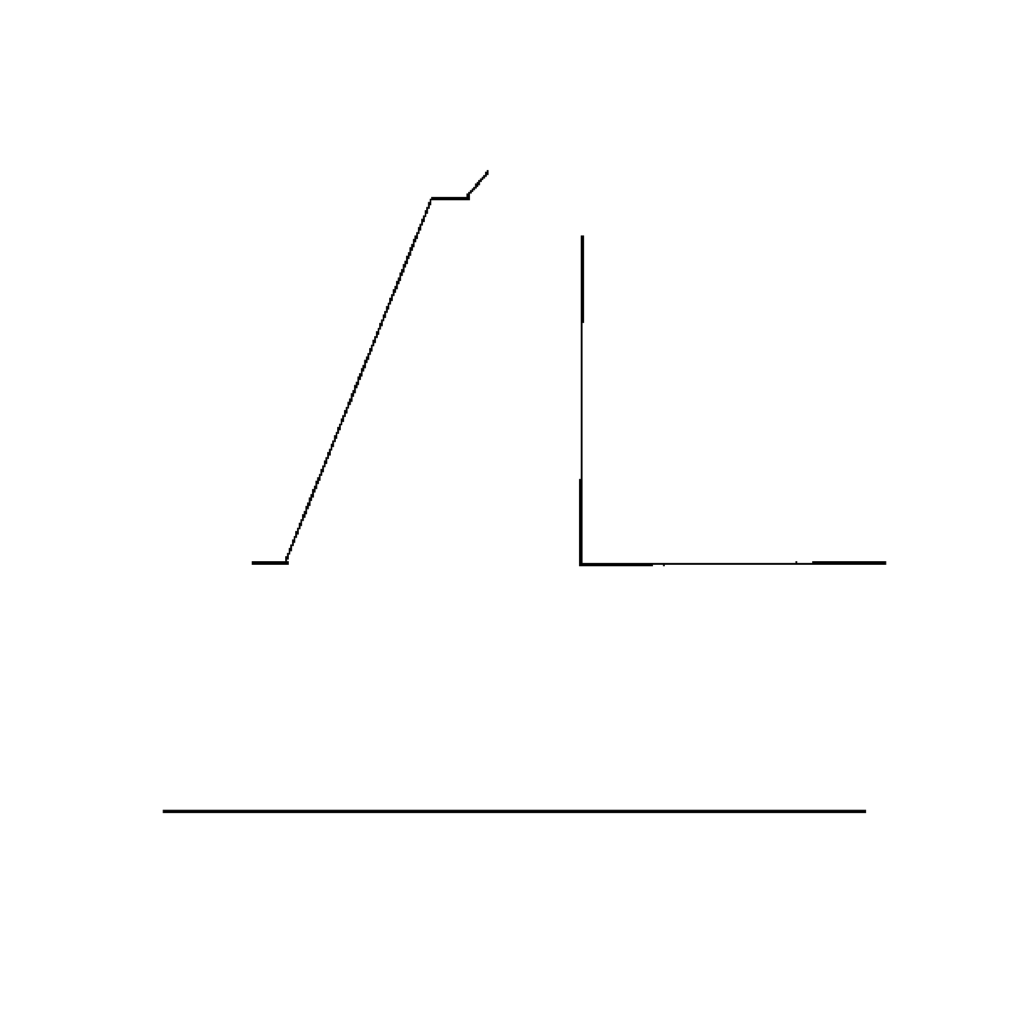
\includegraphics[width=\columnwidth]{synthetic.png}}\end{center}

\title{\LARGE \bf
Compressed Directional Distance Transform for Fast 2D Ray Casting
}


\author{Corey H. Walsh$^{1}$ and Sertac Karaman$^{2}$% <-this % stops a space
% \thanks{*This work was not supported by any organization}% <-this % stops a space
\thanks{$^{1}$Corey H. Walsh is with the Department of Computer Science and Engineering, Massachusetts Institute of Technology,
        Cambridge, MA 02139, USA
        {\tt\small chwalsh@mit.edu}}%
\thanks{$^{2}$Sertac Karaman is with the Laboratory for Information and Decision Systems, Massachusetts Institute of Technology,
        Cambridge, MA 02139, USA
        {\tt\small sertac@mit.edu}}%
}

\begin{document}

\maketitle
\thispagestyle{empty}
\pagestyle{empty}


\skcomment{}{I would consider putting the word ``localization'' in the title.}

%%%%%%%%%%%%%%%%%%%%%%%%%%%%%%%%%%%%%%%%%%%%%%%%%%%%%%%%%%%%%%%%%%%%%%%%%%%%%%%%
\begin{abstract}


Lorem Ipsum is simply dummy text of the printing and typesetting industry. Lorem Ipsum has been the industry's standard dummy text ever since the 1500s, when an unknown printer took a galley of type and scrambled it to make a type specimen book. It has survived not only five centuries, but also the leap into electronic typesetting, remaining essentially unchanged. It was popularised in the 1960s with the release of Letraset sheets containing Lorem Ipsum passages, and more recently with desktop publishing software like Aldus PageMaker including versions of Lorem Ipsum.


\end{abstract}


%%%%%%%%%%%%%%%%%%%%%%%%%%%%%%%%%%%%%%%%%%%%%%%%%%%%%%%%%%%%%%%%%%%%%%%%%%%%%%%%
\section{Introduction}

Determining a robot's location and orientation in a known environment, also known as localization, is an important and challenging problem in the field of robotics. Particle filters are a popular class of Monte Carlo algorithms used to track the pose of mobile robots by iteratively refining a set of pose hypotheses called particles. After determining an initial set of particles, the particle filter updates the position and orientation of each particle by applying a movement model based on available odometry data. Next, the belief in each particle is updated by comparing sensor readings to a map of the environment. Finally, the particles are resampled according to the belief distribution and algorithm repeats.

While particle filters provide a robust and general framework for solving the localization problem, they can be computationally expensive due to both the number of particles which must be maintained and the evaluation of the sensor model. In robots with range sensors such as LiDAR or Sonar, ray casting is frequently used to compare sensor readings with the ground truth distance between the hypothesis pose and obstacles in a map. Ray casting itself is a complex operation, and reweighting any single particle may require tens of ray casts. Many effective particle filters maintain thousands of particles, updating each particle tens of times per second. As a result, millions of ray cast operations may be resolved per second, posing a significant computational challenge for resource constrained systems.

Several well known algorithms exist for ray casting in two dimensional spaces such as Bresenham's Line algorithm \cite{bresenham} and ray marching \cite{raymarching}. Both algorithms work by iteratively checking points in the map starting at the query point and moving in the ray direction until an obstacle is discovered. This process may require hundreds of memory reads per ray cast depending on the distance to the nearest obstacle, and does not provide constant time performance. 

To combat the computational challenges of ray casting while localizing in a two-dimensional map, Thrun et al. \cite{localization} suggest the use of a large three-dimensional lookup table (LUT) to store expected ranges for each discrete $(x,y,\theta)$ state. While this is simple to implement and does result in large speed improvements as compared to ray casting, it can be prohibitively memory intensive for large maps and/or resource constrained systems. In a 2000 by 2000 occupancy map, storing ranges for 200 discrete directions would require over 1.5GB. While this memory requirement may be acceptable in many cases, it scales with the square of map size - a 4000 by 4000 map would require over 6GB for the same angular discretization.

We propose an analogous data structure to the three-dimensional LUT called a Compressed Directional Distance Transform (CDDT) which requires significantly less memory and precomputation time while still allowing near constant time ray casting queries. The contributions of this work are the following. Firstly, we develop a problem formulation and provide details of our method. Secondly, we implement the proposed algorithm and compare its performance to alternate two-dimensional ray casting methods. Finally, we discuss potential extensions to the CDDT algorithm which could be the basis of future research. We observe two orders of magnitude improvement in memory requirements, with little sacrifice in computation time, when compared to the lookup table methods. Additionally, we observe a large speedup when compared to the other ray casting methods considered with similar memory requirements.

\section{Related Work}

Due to varied handling of edge cases and ambiguities in the problem of determining distance between any point and the nearest obstacle in a particular direction, most 2D ray casting algorithms do not provide exactly consistent results for every query. However, on average error between results from each of the methods discussed is small.

Bresenham's line algorithm \cite{bresenham} incrementally determines the set of pixels that approximate the trajectory of query ray starting from the query point $(x,y)$ and progressing in the $\theta$ direction one pixel at a time. The algorithm terminates once the nearest occupied pixel is discovered, and the euclidean distance between that occupied pixel and the query $(x,y)$ is reported. This algorithm is widely implemented in particle filters due to its simplicity and ability to operate on a dynamic map. The primary disadvantage is that it is slow, potentially requiring hundreds of memory accesses for a single ray cast. While actual performance is highly environment dependent, Bresenham’s Line algorithm is linear in map size in the worst case.

Similar to Bresenham's Line algorithm, ray marching \cite{raymarching} checks points along the line radiating outwards from the query point until an obstacle is encountered. The primary difference is that ray marching makes larger steps along the query ray, thereby avoiding unnecessary memory reads. Beginning at the query point $(x,y)$ the ray marching algorithm proceeds in the theta direction, stepping along the line by the minimum distance between each query point and the nearest obstacle. The algorithm terminates when the query point coincides with an obstacle in the map. A precomputed euclidean distance transform of the occupancy map provides the distance between each query point and the nearest obstacle in any direction.

\begin{figure}[h]
\img{spheretrace.jpg}
\caption{Visualization of ray marching starting at $p_0$ towards $p_4$. Green circle around each query point represents the distance to the nearest obstacle from that point. Blue dots represent the query points, labeled in order of execution. From \cite{sphere:source}.}
\label{spheres}
\end{figure}

Ray marching is on average much faster than Bresenham’s line, but edge cases exist in which the performance is nearly equivalent. As noted in \cite{acceleratedraymarching} the traversal speed of rays rapidly decreases as sampled positions approach obstacles. For this reason, rays which travel parallel to walls progress very slowly as compared to those passing through open areas. Thus the performance of ray marching exhibits a long tail distribution as seen in (Fig. \ref{violin:basement:all}, \ref{violin:basement:particle}) which negatively impacts average runtime as compared to the median, and can be problematic for near real time algorithms.

As previously described, a common acceleration technique for two dimensional ray casting is to precompute the ray distances for every state in a discrete grid and store the results in a three dimensional LUT. Any ray casting technique may be used to compute the table. In the authors’ implementation ray casting is used to populate the LUT since it has low initialization time and is significantly faster than Bresenham’s Line. Theoretically this approach has constant query runtime, though actual performance is dependent on access patterns as CPU caching effects are significant in practice.

State space discretization implies approximate results, since intermediate states must be rounded onto the discrete grid. While the effect of rounding query position, it can be significant for $\theta$. As the ray moves further away from the query point along the theta direction, angular discretization error accumulates. For queries $(x,y,\theta)$ discretized into $(x_d,y_d,\theta_d)$, the distance between the end of the ray $(x_d,y_d,Θ_d)$ and its projection onto the line implied by $(x,y,\theta)$ becomes large as the length of the ray increases. Although the error induced by discretization may be unacceptable for computer graphics applications, it is generally acceptable for probabilistic algorithms such as the particle filter since error is expected and directly modeled. 

Rather than simply rounding to the nearest grid state, one method to improve accuracy of queries which lie between discrete states is to query the neighboring states and interpolate between them. Since we are evaluating the performance of these methods for use in a particle filter, we do not perform interpolation since the increased computation reduces the number of particles that may be maintained in real time, and therefore any increase in accuracy with respect to the stored map is effectively negated.

\section{Problem Formulation and Notation}

We define the problem of ray casting in occupancy grids as follows. We assume a known occupancy grid map in which occupied cells have value one and unoccupied cells have value zero. Given a query pose $(x,y,\theta)_{query}$ in map space, the ray cast operation finds the nearest occupied pixel $(x,y)_{collide}$ which lies on the ray starting at the position $(x,y)_{query}$ pointing in the $\theta_{query}$ direction. The ray cast operation returns the euclidean distance $d_{ray}$ between $(x,y)_{query}$ and $(x,y)_{collide}$.

$$ d_{ray} = \left\Vert\begin{pmatrix}
           x \\
           y 
         \end{pmatrix}_{query} - 
         \begin{pmatrix}
           x \\
           y
         \end{pmatrix}_{collide}\right\Vert_2
$$

We refer to $(x,y,\theta)_{query}$ as the query pose, and $(x,y)_{query}$ as the query point. Additionally, denote the discretized query pose as $\lfloor(x,y,\theta)_{query}\rceil$. A $\theta$ slice through the LUT refers to all table entries for that particular $\lfloor\theta\rceil$.

\begin{figure}[h]
\img{coord_system.png}
\caption{Occupancy grid map coordinate system}
\label{coordinate_system}
\end{figure}

\section{The Compressed Directional Distance Transform Algorithm}

Although the three dimensional table used to store precomputed ray cast solutions for a discrete state space is inherently large, it is highly compressible. This is most apparent in the cardinal directions, in which adjacent values along a particular dimension of the table increase by exactly one unit of distance for unobstructed positions as in Fig. \ref{cardinal_example}. Our data structure is designed to compress this redundancy while still allowing for fast queries in near constant time. We accomplish this though through what we refer to as a Compressed Directional Distance Transform (CDDT) described here.

\begin{figure}[h]
\begin{center}
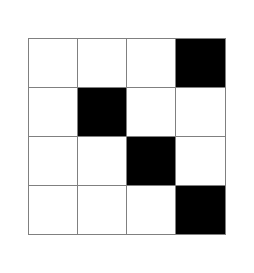
\begin{tikzpicture}
\fill[black,scale=\gridScale] (0.5,0.5) rectangle (1,1);
\fill[black,scale=\gridScale] (-0.5,0) rectangle (0,0.5);
\fill[black,scale=\gridScale] (0,-0.5) rectangle (0.5,0);
\fill[black,scale=\gridScale] (0.5,-1) rectangle (1,-0.5);
\draw[scale=\gridScale,step=0.5cm,color=white] (-1,-1.1) grid (1,1.1);
\draw[scale=\gridScale,step=0.5cm,color=gray] (-1,-1) grid (1,1);
\end{tikzpicture}
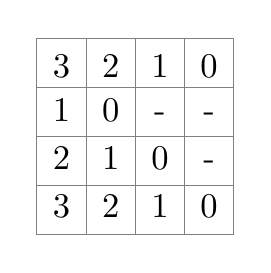
\begin{tikzpicture}
\draw[scale=\gridScale,step=0.5cm,color=white] (-1,-1.1) grid (1,1.1);
\draw[scale=\gridScale,step=0.5cm,color=gray] (-1,-1) grid (1,1);
\matrix[matrix of nodes,nodes={inner sep=0pt,text width=.5cm,align=center,minimum height=0.45cm, scale=\gridScale}]{
3 & 2 & 1 & 0 \\
1 & 0 & - & - \\
2 & 1 & 0 & - \\    
3 & 2 & 1 & 0\\};
\end{tikzpicture}
\end{center}
\caption{Occupancy grid (left) and associated LUT for $\theta=0$ (right).}
\label{cardinal_example}
\end{figure}

The euclidean distance transform of an occupancy grid map stores the distance to the nearest obstacle in any direction $\theta$ for each possible $\lfloor(x,y)\rceil$ in the map. In contrast, a directional distance transform (DDT) stores the distance to the nearest obstacle in a particular direction $\lfloor\theta\rceil$ for every $\lfloor(x,y)\rceil$. The key difference between a single $\theta$ slice of the LUT and a directional distance transform for the same $\theta$ is the way in which it is computed and indexed. To compute the LUT slice, ray casting is performed in the $\theta$ direction for every $\lfloor(x,y)\rceil$. At runtime, each $(x,y)_{query}$ is discretized to $\lfloor(x,y)_{query}\rceil$ and the LUT slice is directly indexed.

In contrast, to compute the DDT, the obstacles in the map are rotated about the origin by $-\lfloor\theta\rceil$ and ray casting is implicitly performed in the $\theta=0$ direction to populate the table. Then, to index the table for a query $(x,y,\theta)_{query}$ one discretizes to $\lfloor(x,y,\theta)_{query}\rceil$, rotates $\lfloor(x,y)_{query}\rceil$ about the origin, and uses the rotated coordinates $\lfloor(x,y,\theta)_{query}\rceil_{rot}$ to index into the DDT. Thus, the same operation is computed in both the DDT and the LUT, but while one changes the ray cast direction to populate the LUT, one rotates scene geometry and ray casts in a constant direction to populate the DDT. While it is true that the rotation of the scene geometry introduces small errors as compared to ray casting for each cell, as previously discussed small errors do not significantly impact particle filter localization performance due to the use of a probabilistic error model and are dominated by errors inherently present in distance sensors. 

The distinction between the LUT slice and the DDT may be subtle, but it has an important effect. Since ray casting is always performed in the $\theta=0$ direction to populate the DDT, all values in the same row of the DDT either increase by one unit with respect to their neighbor in the $\theta=0$ direction or go to zero. Thus each row of the DDT may be characterized as a sawtooth function where the zero points correspond to obstacles in the map. This characterization as a sawtooth function provides a natural method of lossless compression: keep the zero points and discard the rest.

The conversion from a DDT to a CDDT slice is performed by storing the $x$ coordinate of each zero point in the coordinate space of the DDT for every discrete row. At query time, the sawtooth function (which is the distance to the nearest obstacle in the query direction) encoded in the DDT may be quickly recovered by performing binary search for nearest zero point in the correct row of the CDDT slice. We refer to the list of zero points for a single row as a CDDT bin. Similar to the LUT, the full CDDT is defined as every CDDT slice for all discrete values of $\theta$.

For performance, it is not necessary to compute the full DDT, but rather the CDDT may be directly constructed by projecting each obstacle into the coordinate space of the DDT for every $\lfloor\theta\rceil$ and sorting its $x$ coordinate in the CDDT bin corresponding to its $y$ coordinate and rotation. After all geometry has been projected into the CDDT, each bin is sorted to facilitate later indexing. Not only does the direct construction of the CDDT greatly reduce the amount of memory required to store the LUT, it also reduces data structure precomputation time since ray casting is not necessary.

[TODO add an example of scene rotation, saw tooth wave, and zero point projection]

\subsection{CDDT Construction Algorithm}

\subsection{CDDT Query Algorithm}


{\color{red}DONE WITH SECOND EDITING PASS UP TO THIS POINT}



Once the CDDT is constructed, querying the data structure to resolve ray casts involves

\begin{enumerate}
    \item Projecting the query point into the coordinate space of the slice which corresponds to the discretized theta
    \item Finding the nearest zero point which has a y-coordinate greater than or equal to the query point in the projected coordinate space
    \item Return the distance between the query point and the nearest zero point in the projected coordinate space, which is simply the difference between y-coordinates
\end{enumerate}

Binary search is theoretically optimal for finding zero points near to query states, in our implementation we conditionally use linear search when the number of zero points is below a certain constant (we use 64) as it has a superior memory access pattern in such cases.
While conceptually simple, implementing the CDDT data structure construction and traversal routines requires careful consideration in order to capture all edge cases and to minimize unnecessary computation. In this sense, it is more complex to implement than the alternatives considered, however there are many opportunities for optimization which yield real-world speed up. To ease this burden, we provide our implementation as well as Python wrappers with an Apache 2.0 license.


\skcomment{}{You can put all the text after this point into one subsection, which you can call ``Further optimizations'' or something like that.}

\subsection{Further Optimizations}

A side effect of extracting the zero points from each column of the DDT is the introduction of rotational symmetry. For any given theta, the zero points accumulated by projecting scene geometry into the requisite coordinate space are mirror images of those accumulated by projecting scene geometry into the theta+pi direction. Therefore, one need only compute the CDDT for the range of discrete thetas from $[0,\pi)$ and the DDT for the range $[0,2\pi)$ may be inferred, resulting in factor of two further reduction in memory usage.

In addition to the aforementioned reduction in memory usage, rotational symmetry may be exploited in scenarios where ray casts are performed radially around a single point. While traversing the data structure to resolve a ray cast in a particular $(x,y,\theta)$, the ray cast for $(x,y,\theta+\pi)$ may be resolved with a single additional memory read. Once the index i of the nearest zero point in the theta direction $z_{\theta}$ is discovered, the index of the nearest zero point in the opposite direction is simply i-1. For example, in robots with laser scanners sweeping angles larger than 180°, this symmetry can be used to reduce the number of data structure traversals required to compute the sensor model by up to a factor of two.

\subsection{Incremental Update}

While the authors did not implement the necessary changes, we conjecture that the CDDT algorithm could be modified to allow incremental updates to the map. In contrast, any change to the map would introduce inconsistencies in a precomputed LUT requiring a full re-computation of the data structure. Ray casting every state in a three dimensional grid is highly computational, ruling out the possibility of using a precomputed LUT with dynamic maps such as in SLAM algorithms. Similarly, ray marching operates on a euclidean distance transform which cannot be easily updated in an incremental fashion. While Bresenham’s line algorithm is the slowest option evaluated in terms of ray cast performance, it has the benefit that it operates directly on the occupancy grid map and can therefore be used with dynamic maps. For this reason, Bresenham’s line is one of the most commonly used algorithms for ray casting in occupancy grids.

To allow incremental update of the CDDT, the sorted vector data structure used in our implementation should be replaced with an alternative which allows for $O(logn)$ insert and delete, such as a randomized skip list. To aid in node deletion, pointers could be maintained from each grid element to the associated leaf node in the randomized skip lists with a constant factor increase in memory usage. 

In this case, the cost of inserting or deleting an occupied grid cell would be \skcomment{$O(theta\_discretization*\log(number of lut bin elements))$.}{I think this is your plan already, but just to note: Please make sure to use symbols for these and introduce what the symbols mean. } The number of elements in each lut bin tends to be small and is bounded, so this becomes $O(theta\_discretization)$ which is likely not prohibitive for real-time performance.

Skip list traversal is likely to be less efficient than binary search on sorted vectors due to worse cache characteristics. However, the authors expect it to still be significantly faster than performing Bresenham’s line, and therefore recommend that this modification be the subject of future research.

\subsection{Pruning}

By removing entries in the CDDT which can never possibly result in a ray collision, it is possible to further reduce the memory footprint of the data structure. \skcomment{Consider a 3x3 block of obstacles in an otherwise empty map.}{I think this deserves a figure, just to allow the reader to quickly read your paper.} The center obstacle will never be the nearest neighbor in any ray casting query, because any such query would first intersect with one of the 8 surrounding obstacles. To exploit this, one can take the morphological edge map of the occupancy grid map prior to CDDT generation without loss of generality. This can result in significant memory usage and data structure construction time reductions in dense maps where the number of obstacles adjacent to empty cells is small compared to the total number of obstacles. Prior to performing ray casting on the CDDT data structure, we check the occupancy grid to ensure that the query point itself is not an obstacle and return a distance of zero if so in order to prevent incorrect results when ray casting from the middle of obstacles which may be removed by the morphological operation.

\begin{figure}[h]
\img{slice0_pcddt_basement.png}
\caption{The same slice of the DDT as \ref{cddt:slice0}. Notice that the number of elements projected into each CDDT bin is less peaky since the pruning operation removes most elements of long lines of obstacles. Also note the higher compression factor of 415 for this slice, increased from 267 in the unpruned CDDT.}
\label{pcddt:slice0}
\end{figure}

\skcomment{Additionally, consider a line of obstacles aligned along the Y-axis.}{While you are at it, put a figure for this one too? } Every element in this line will be projected into a single list of zero points for the theta=0 slice of the CDDT. However, the middle elements of the line will never result in a collision. Any ray cast from adjacent states in the $\theta=0$ direction will return early in the occupancy grid check, and any ray cast from outside the wall will collide with one of the edge-most obstacles in that line. Therefore in the theta=0 slice, one may discard the zero points corresponding to the middle elements without introducing error. This form of optimization is simple to compute in the cardinal directions, but non-trivial for arbitrary theta not aligned with an axis. Rather than attempting to analytically determine which obstacles may be discarded, it is simpler to prune the data structure by ray casting from every possible state (as in the LUT data structure) and discard any zero point which is unused. 

Pruning does also increase precomputation time rendering it incompatible with incremental update, however the reduction of memory usage is worthwhile for static maps. In addition to memory reduction, we find that pruning slightly improves runtime performance, likely as a result of improved caching characteristics.

\skcomment{}{Do you think you can have a subsection called ``analysis'' which has a few propositions/theorems that say things like Memory requirement is $O(NM)$ and running time is $O(1)$? This may be hard given the deadline, but osmething to think about. }


\section{EXPERIMENTS}

We have implemented the proposed algorithm in the C++ programming language, as well as Bresenham’s Line, ray marching, and the LUT approach for comparison. Our source code is available for use and analysis [TODO add a link to github], and Python wrappers are also provided for easier usage. All benchmarks were performed on a desktop computer on a Intel Core i5-4590 CPU @ 3.30GHz with 16GB DDR3 ram @ 1333MHz, running Ubuntu 14.04.


\begin{figure}[ht]
\img{basement_grid_random_cropped.png}
% \begin{center}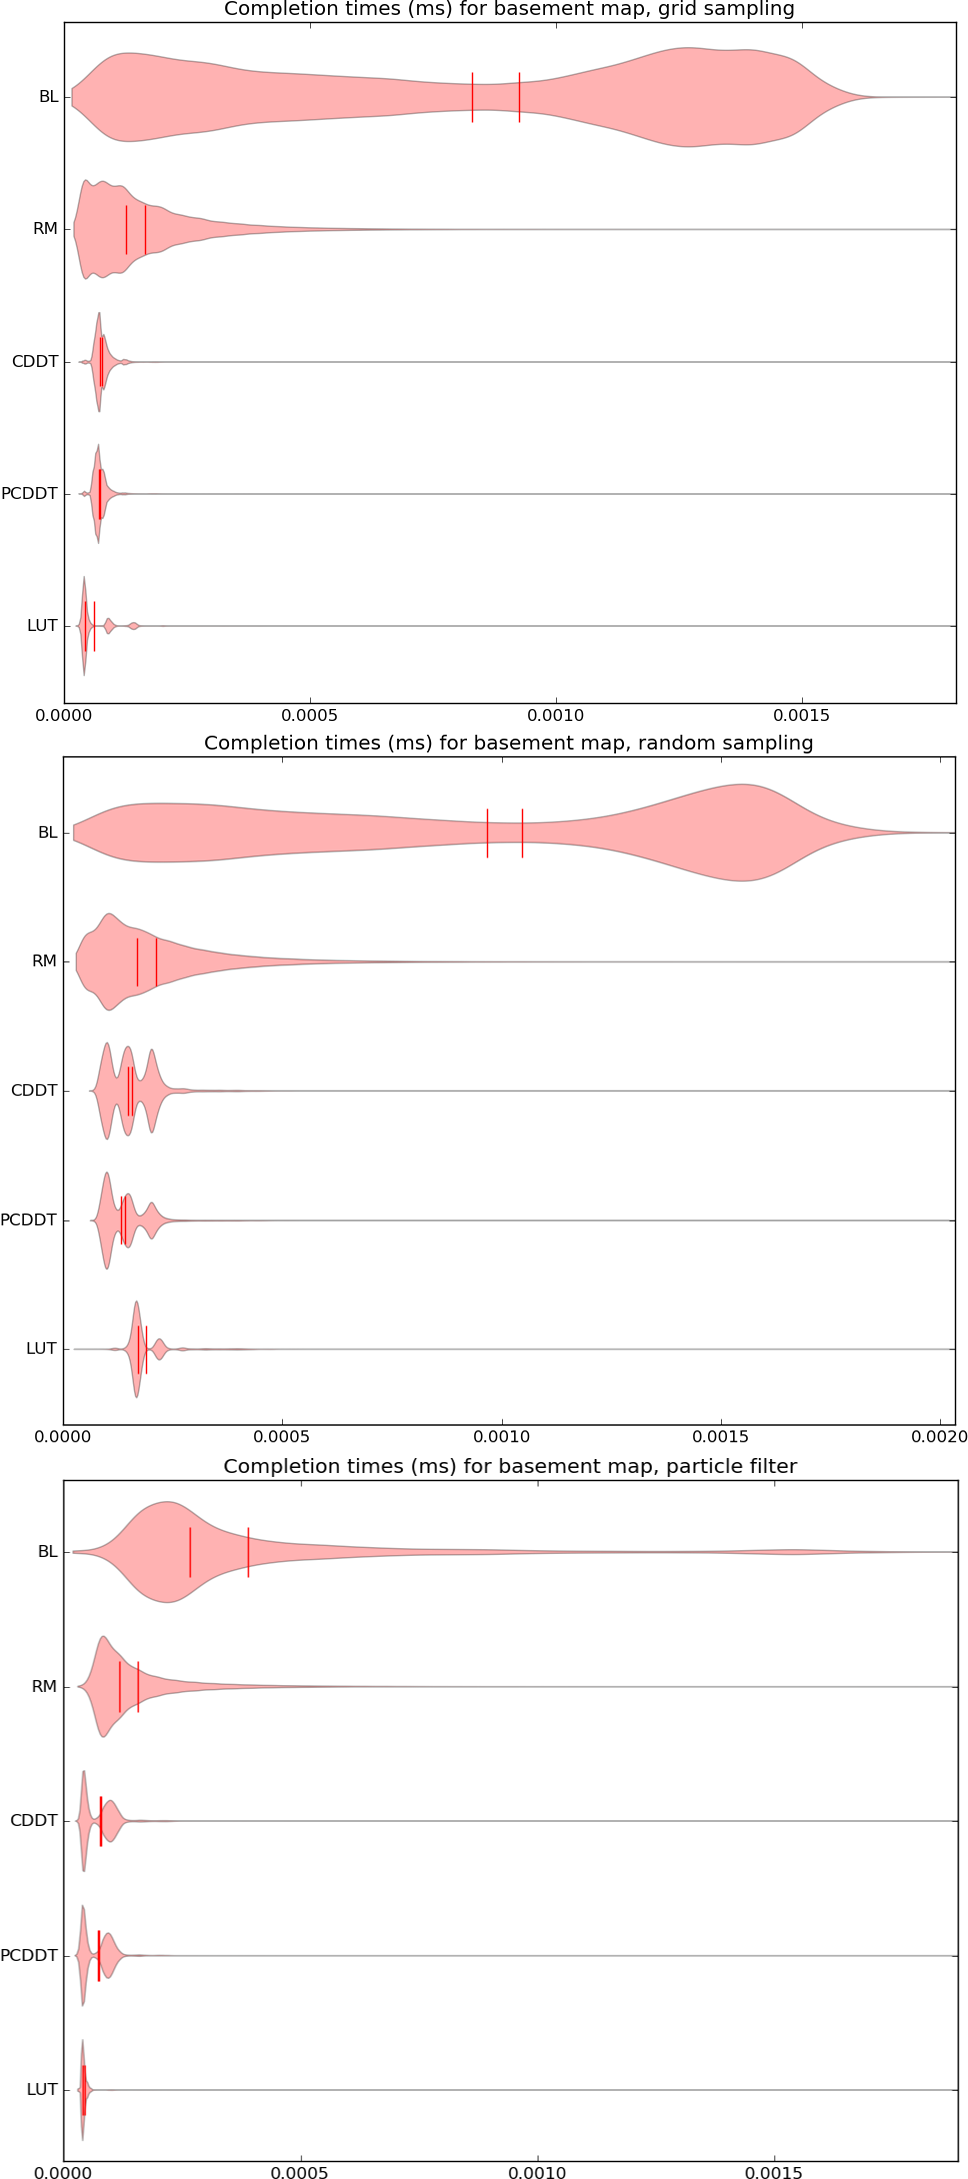
\includegraphics[width=248px,height=520px]{basement_benchmarks_cropped.png}\end{center}
\caption{Violin plots demonstrating histogram of completion time over a large number of queries for each ray cast method. Basement map. X axis shows time in milliseconds, and Y axis shows the number of queries that completed after that amount of time.}
\label{violin:basement:all}
\end{figure}

\subsection{Synthetic Benchmarks}

% \begin{figure}[h]
% \img{grid_trial2_basement_cropped.png}
% \caption{Violin plots demonstrating histogram of completion time over a large number of queries for each ray cast method. Basement map. X axis shows time in milliseconds, and Y axis shows the number of queries that completed after that amount of time.}
% \label{violin:basement:grid}
% \end{figure}

% \begin{figure}[h]
% \img{grid_trial2_synthetic_cropped.png}
% \caption{Violin plots demonstrating histogram of completion time over a large number of queries for each ray cast method. Synthetic map. X axis shows time in milliseconds, and Y axis shows the number of queries that completed after that amount of time.}
% \label{violin:basement:grid}
% \end{figure}

% \begin{figure}[h]
% \img{random_trial2_basement_cropped.png}
% \caption{Violin plots for a large number of randomly sampled queries. Basement map. The random access pattern degrades the caching performance variably for each method.}
% \label{violin:basement:random}
% \end{figure}

% \begin{figure}[h]
% \img{random_trial2_synthetic_cropped.png}
% \caption{Violin plots for a large number of randomly sampled queries. Synthetic map. The random access pattern degrades the caching performance variably for each method.}
% \label{violin:basement:random}
% \end{figure}

We evaluate algorithm performance in two synthetic benchmarks, using two different maps. The so called Synthetic map was created with photoshop, whereas the basement map was created via a SLAM algorithm on the RACECAR platform [cite this?]. The first benchmark computes a ray cast for each point in a uniformly spaced grid over the three dimensional state space. The second benchmark performs a large number of ray casts for randomly generated states.

\begin{figure}[ht]
\begin{center}
\begin{tabular}{ | m{8em} | m{2.3cm}| m{1.5cm} | } 
\hline
 \multicolumn{3}{|c|}{Basement Map, $\theta$ discretization: 108} \\
 \hline
 Method & Memory Usage & Init. Time \\
 \hline
 Bresenham's Line & 1.37 MB & 0.006 sec  \\
 Ray Marching & 5.49 MB & 0.16 sec  \\
 CDDT & 6.34 MB & 0.067 sec  \\
 PCDDT & 4.07 MB & 2.2 sec  \\
 Lookup Table & 296.63 MB & 15.3 sec  \\
\hline
\end{tabular}
\end{center}
\caption{The construction time and memory footprint of each method for the Basement map.}
\label{table:basement:init}
\end{figure}

\begin{figure}[ht]
\begin{center}
\begin{tabular}{ | m{8em} | m{2.3cm}| m{1.5cm} | } 
\hline
 \multicolumn{3}{|c|}{Synthetic Map, $\theta$ discretization: 108} \\
 \hline
 Method & Memory Usage & Init. Time \\
 \hline
 Bresenham's Line & 1 MB & 0.004 sec  \\
 Ray Marching  & 4 MB & 0.13 sec  \\
 CDDT & 2.71 MB & 0.03 sec  \\
 PCDDT & 1.66 MB & 0.74 sec  \\
 Lookup Table & 216 MB & 9.1 sec  \\
\hline
\end{tabular}
\end{center}
\caption{The construction time and memory footprint of each method for the Synthetic map.}
\label{table:synthetic:init}
\end{figure}

\subsection{Particle Filter Experiments}

\begin{figure}[h]
\img{particle_trial2_basement_cropped.png}
\caption{Violin plots for ray casting completion times during the execution of a particle filter. Basement map. Ray casting is primarily done inside of hallways, reducing the mean ray length and thereby improving Bresenham's Line performance. CDDT and PCDDT exploiting radial symmetry while resolving the sensor model.}
\label{violin:basement:particle}
\end{figure}

To simulate real world operating conditions, we have implemented a particle filter localization algorithm using a beam mode sensor model. We provide statistics about the ray cast performance of each algorithm while being used to compute the sensor model, as well as end to end statistics on the number of particles able to be maintained in real-time. While care was taken in implementing the particle filter, there are undoubtedly many optimizations which could further improve end-to-end performance. Thus, these benchmarks should not be considered an upper bound on performance and should be interpreted comparatively.

Our sensor model is designed for the Hokuyo UST-10LX lidar scanner used aboard the RACECAR platform [cite this?], which features a 270° field of view. Since this FOV is in excess of 180° we exploit radial symmetry discussed in [radial symmetry section] to simultaneously ray cast in the theta and $\theta+180°$ direction when possible. As demonstrated in the below figure, this optimization reduces the number of data structure traversals required by a third as compared to the other methods evaluated, while still resolving the same number of ray casts. As is standard in such applications, we downsample the resolution of the laser scanner to reduce the number of ray casts per sensor model evaluations and to make the probability distribution over the state space less peaked.

\section{CONCLUSIONS}

This work demonstrates that the proposed CDDT algorithm may be used in mobile robotics to accelerate sensor model computation when localizing in a two dimensional occupancy grid map. While the precomputed LUT approach is generally 1.1 to 1.7 times faster than the proposed algorithm, the memory footprint of the proposed data structure is significantly smaller which may be desirable for resource constrained systems. Other than the LUT approach, CDDT is significantly faster than the other methods evaluated. Ray marching is the next best, ranging from 1.28 to 2.25 times slower than PCDDT depending on access patterns and environmental factors. The comparison with the widely used Bresenham's Line algorithm is more stark, ranging from a factor of 5.39 to 14.8 in our benchmarks.

In future work we aim to further develop our approach to allow for incremental map updates without requiring a full reconstruction of the underlying acceleration data structure, a feature which currently only the slowest evaluated method supports.

\addtolength{\textheight}{-12cm}   % This command serves to balance the column lengths
                                  % on the last page of the document manually. It shortens
                                  % the textheight of the last page by a suitable amount.
                                  % This command does not take effect until the next page
                                  % so it should come on the page before the last. Make
                                  % sure that you do not shorten the textheight too much.

%%%%%%%%%%%%%%%%%%%%%%%%%%%%%%%%%%%%%%%%%%%%%%%%%%%%%%%%%%%%%%%%%%%%%%%%%%%%%%%%



%%%%%%%%%%%%%%%%%%%%%%%%%%%%%%%%%%%%%%%%%%%%%%%%%%%%%%%%%%%%%%%%%%%%%%%%%%%%%%%%



%%%%%%%%%%%%%%%%%%%%%%%%%%%%%%%%%%%%%%%%%%%%%%%%%%%%%%%%%%%%%%%%%%%%%%%%%%%%%%%%
\section*{APPENDIX}

\begin{figure}[h!]
\img{synthetic_cropped.png}
\caption{Synthetic map occupancy grid. 1024x1024}
\label{violin:basement:grid}
\end{figure}

\begin{figure}[h!]
\begin{center}
\newcolumntype{C}[1]{>{\centering\arraybackslash}m{#1}}
\begin{tabular}{ | C{1.15cm} | C{1.25cm}| C{1.25cm} | C{1.25cm} | C{1.25cm}|  } 
\hline
\multicolumn{5}{|c|}{\textbf{Synthetic Map Ray Cast Benchmarks}} \\
\hline \hline
\multicolumn{5}{|c|}{Random Sampling} \\
\hline
Method & Mean & Median & IQR & Speedup \\
\hline
BL & 1.19e-06 & 1.41e-06 & 7.71e-07 & 1 \\
RM & 1.52e-07 & 1.25e-07 & 1.05e-07 & 7.81 \\
CDDT & 1.24e-07 & 1.05e-07 & 5.3e-08 & 9.59 \\
PCDDT & 1.19e-07 & 1.01e-07 & 5e-08 & 10.02 \\ 
LUT & 1.82e-07 & 1.68e-07 & 1.4e-08 & 6.55 \\
\hline \hline
\multicolumn{5}{|c|}{Grid Sampling} \\
\hline
Method & Mean & Median & IQR & Speedup \\
\hline
BL & 1.03e-06 & 1.20e-06 & 6.79e-07 & 1 \\ 
RM & 1.27e-07 & 1.03e-07 & 1.06e-07 & 8.06 \\
CDDT & 7.02e-08 & 6.8e-08 & 1e-08 & 14.63 \\
PCDDT & 6.94e-08 & 6.8e-08 & 9e-09 & 14.80 \\
LUT & 6.33e-08 & 4.2e-08 & 4.6e-08 & 16.21 \\
\hline
\end{tabular}
\caption{All times listed in seconds, speedup relative to Bresenham's Line}
\label{table:basement:init}
\end{center}
\end{figure}



\begin{figure}[h!]
\begin{center}
\newcolumntype{C}[1]{>{\centering\arraybackslash}m{#1}}
\begin{tabular}{ | C{1.15cm} | C{1.25cm}| C{1.25cm} | C{1.25cm} | C{1.25cm}|  } 
\hline
\multicolumn{5}{|c|}{\textbf{Basement Map Ray Cast Benchmarks}} \\
\hline \hline
Method & Mean & Median & IQR & Speedup \\
\hline
\multicolumn{5}{|c|}{Random Sampling} \\
\hline
BL & 9.66e-07 & 1.05e-06 & 1.08e-06 & 1 \\
RM & 2.12e-07 & 1.68e-07 & 1.64e-07 & 4.56 \\
CDDT & 1.58e-07 & 1.49e-07 & 9.1e-08 & 6.13 \\
PCDDT & 1.41e-07 & 1.32e-07 & 6.5e-08 & 6.83 \\
LUT & 1.89e-07 & 1.7e-07 & 2.1e-08 & 5.10 \\
\hline \hline
\multicolumn{5}{|c|}{Grid Sampling} \\
\hline
Method & Mean & Median & IQR & Speedup \\
\hline
BL & 8.29e-07 & 9.24e-07 & 9.53e-07 & 1 \\
RM & 1.65e-07 & 1.26e-07 & 1.34e-07 & 5.02 \\
CDDT & 7.69e-08 & 7.2e-08 & 1.6e-08 & 10.78 \\
PCDDT & 7.32e-08 & 7e-08 & 1.4e-08 & 11.33 \\
LUT & 6.13e-08 & 4.3e-08 & 4.6e-08 & 13.53 \\
\hline \hline
\multicolumn{5}{|c|}{Particle Filter} \\
\hline
Method & Mean & Median & IQR & Speedup \\
\hline
BL & 3.89e-07 & 2.67e-07 & 2.31e-07 & 1 \\
RM & 1.56e-07 & 1.18e-07 & 9.4e-08 & 2.49 \\
CDDT & 7.67e-08 & 7.8e-08 & 5.7e-08 & 5.07 \\
PCDDT & 7.22e-08 & 7.4e-08 & 5.4e-08 & 5.39 \\
LUT & 4.35e-08 & 4.1e-08 & 5e-09 & 8.94 \\
\hline
\end{tabular}

\caption{All times listed in seconds, speedup relative to Bresenham's Line}
\label{table:basement:init}
\end{center}
\end{figure}





% \begin{figure}[h!]
% \begin{center}
% \begin{tabular}{ | m{1.05cm} | m{1.3cm}| m{1.6cm} | m{1.25cm} | m{1.25cm}|  } 
% \hline
% \multicolumn{5}{|c|}{Basement Map, Random Sampling Ray Cast} \\
% \hline
% Method & Mean & Median & IQR & Speedup \\
% \hline
% BL & 9.66e-07 & 1.05e-06 & 1.08e-06 & 1 \\
% RM & 2.12e-07 & 1.68e-07 & 1.64e-07 & 4.56 \\
% CDDT & 1.58e-07 & 1.49e-07 & 9.1e-08 & 6.13 \\
% PCDDT & 1.41e-07 & 1.32e-07 & 6.5e-08 & 6.83 \\
% LUT & 1.89e-07 & 1.7e-07 & 2.1e-08 & 5.10 \\
% \hline
% \end{tabular}
% \end{center}
% \caption{Statistics per ray cast query for random sampling synthetic map.}
% \label{table:basement:init}
% \end{figure}
% \begin{figure}[h!]
% \begin{center}
% \begin{tabular}{ | m{1.05cm} | m{1.3cm}| m{1.6cm} | m{1.25cm} | m{1.25cm}|  } 
% \hline
% \multicolumn{5}{|c|}{Basement Map, Grid Sampling Ray Cast} \\
% \hline
% Method & Mean & Median & IQR & Speedup \\
% \hline
% BL & 8.29e-07 & 9.24e-07 & 9.53e-07 & 1 \\
% RM & 1.65e-07 & 1.26e-07 & 1.34e-07 & 5.02 \\
% CDDT & 7.69e-08 & 7.2e-08 & 1.6e-08 & 10.78 \\
% PCDDT & 7.32e-08 & 7e-08 & 1.4e-08 & 11.33 \\
% LUT & 6.13e-08 & 4.3e-08 & 4.6e-08 & 13.53 \\
% \hline
% \end{tabular}
% \end{center}
% \caption{Statistics per ray cast query for grid sampling synthetic map.}
% \label{table:basement:init}
% \end{figure}
% \begin{figure}[h!]
% \begin{center}
% \begin{tabular}{ | m{1.05cm} | m{1.3cm}| m{1.6cm} | m{1.25cm} | m{1.15cm}|  } 
% \hline
% \multicolumn{5}{|c|}{Basement Map, Particle Filter Ray Cast} \\
% \hline
% Method & Mean & Median & IQR & Speedup \\
% \hline
% BL & 3.89e-07 & 2.67e-07 & 2.31e-07 & 1 \\
% RM & 1.56e-07 & 1.18e-07 & 9.4e-08 & 2.49 \\
% CDDT & 7.67e-08 & 7.8e-08 & 5.7e-08 & 5.07 \\
% PCDDT & 7.22e-08 & 7.4e-08 & 5.4e-08 & 5.39 \\
% LUT & 4.35e-08 & 4.1e-08 & 5e-09 & 8.94 \\
% \hline
% \end{tabular}
% \end{center}
% \caption{Statistics per ray cast query for random sampling basement map.}
% \label{table:basement:init}
% \end{figure}
% \begin{figure}[h!]
% \begin{center}
% \begin{tabular}{ | m{1.05cm} | m{1.3cm}| m{1.6cm} | m{1.25cm} | m{1.15cm}|  } 
% \hline
% \multicolumn{5}{|c|}{Synthetic Map, Random Sampling Ray Cast} \\
% \hline
% Method & Mean & Median & IQR & Speedup \\
% \hline
% BL & 1.19e-06 & 1.41e-06 & 7.71e-07 & 1 \\
% RM & 1.52e-07 & 1.25e-07 & 1.05e-07 & 7.81 \\
% CDDT & 1.24e-07 & 1.05e-07 & 5.3e-08 & 9.59 \\
% PCDDT & 1.19e-07 & 1.01e-07 & 5e-08 & 10.02 \\ 
% LUT & 1.82e-07 & 1.68e-07 & 1.4e-08 & 6.55 \\
% \hline
% \end{tabular}
% \end{center}
% \caption{The construction time and memory footprint of each method for the Basement map.}
% \label{table:basement:init}
% \end{figure}
% \begin{figure}[h!]
% \begin{center}
% \begin{tabular}{ | m{1.05cm} | m{1.3cm}| m{1.6cm} | m{1.25cm} | m{1.15cm}|  } 
% \hline
% \multicolumn{5}{|c|}{Synthetic Map, Grid Sampling Ray Cast} \\
% \hline
% Method & Mean & Median & IQR & Speedup \\
% \hline
% BL & 1.03e-06 & 1.20e-06 & 6.79e-07 & 1 \\ 
% RM & 1.27e-07 & 1.03e-07 & 1.06e-07 & 8.06 \\
% CDDT & 7.02e-08 & 6.8e-08 & 1e-08 & 14.63 \\
% PCDDT & 6.94e-08 & 6.8e-08 & 9e-09 & 14.80 \\
% LUT & 6.33e-08 & 4.2e-08 & 4.6e-08 & 16.21 \\
% \hline
% \end{tabular}
% \end{center}
% \caption{The construction time and memory footprint of each method for the Basement map.}
% \label{table:basement:init}
% \end{figure}

\begin{thebibliography}{99}

\bibitem{localization} Sebastian Thrun, Dieter Fox, Wolfram Burgard and Frank Dellaert. “Robust Monte Carlo Localization for Mobile Robots.” Artificial Intelligence Journal. 2001

\bibitem{bresenham} J. Bresenham, “Algorithm for Computer Control of a Digital Plotter,” IBM Systems Journal, vol. 4, no. 1, pp. 25-30, 1965

\bibitem{raymarching} K. Perlin and E. M. Hoffert, “Hypertexture.” Computer Graphics, vol 23, no. 3, pp. 297-306, 1989.

\bibitem{acceleratedraymarching} Zuiderveld, Karel, Koning, Anton, and Viergever, Max, “Acceleration of ray-casting using 3D distance transforms”, Proceedings of the SPIE – Visualization in Biomedical Computing 1992, Vol.1808, pp.324-335, 1992.
 
\bibitem{sphere:source} Pharr, M., and R. Fernando. GPU Gems 2: Programming Techniques for High-Performance Graphics and General-Purpose Computation: Addison Wesley Professional. 2005. http://http.developer.nvidia.com/GPUGems2/gpugems2\_chapter08.html

\end{thebibliography}







\end{document}